\section{Simulation Results}
In this section we simulate one MT865 tractor using the newly derived multi body vehicle model. Figure \ref{fig:MB_Tractor_2D_Plot} shows the path traversed along with snapshots of position for initial and terminal simulation positions. Figure \ref{fig:MB_Tractor_traj} shows plots of vehicle speed $v_T = \sqrt{v_x^2 + v_y^2}$, yaw rate $\dot\theta$, left and right slip ratios $i_L$ and $i_R$, engine speed $\Omega_E$ and drawbar arm angle $\phi$. The initial $[X,Y]$ starting locations for the tractor is $[120, 210]$. The manned leader's trajectory is dictated using a combination of open loop and closed-loop commands. Open loop commands include throttle , $\Pi_{leader} = [0.9, 0.9  ,0.9, 0.98]^T$, and gear selections, $g_{GR,leader} = [ 9 , 10 , 11 , 12]^T$, for the time vector $t = [0 , 3 , 8 , 20]^T$ seconds. 
\begin{figure}[htbp]
    \centering
    \vspace{-15pt}
    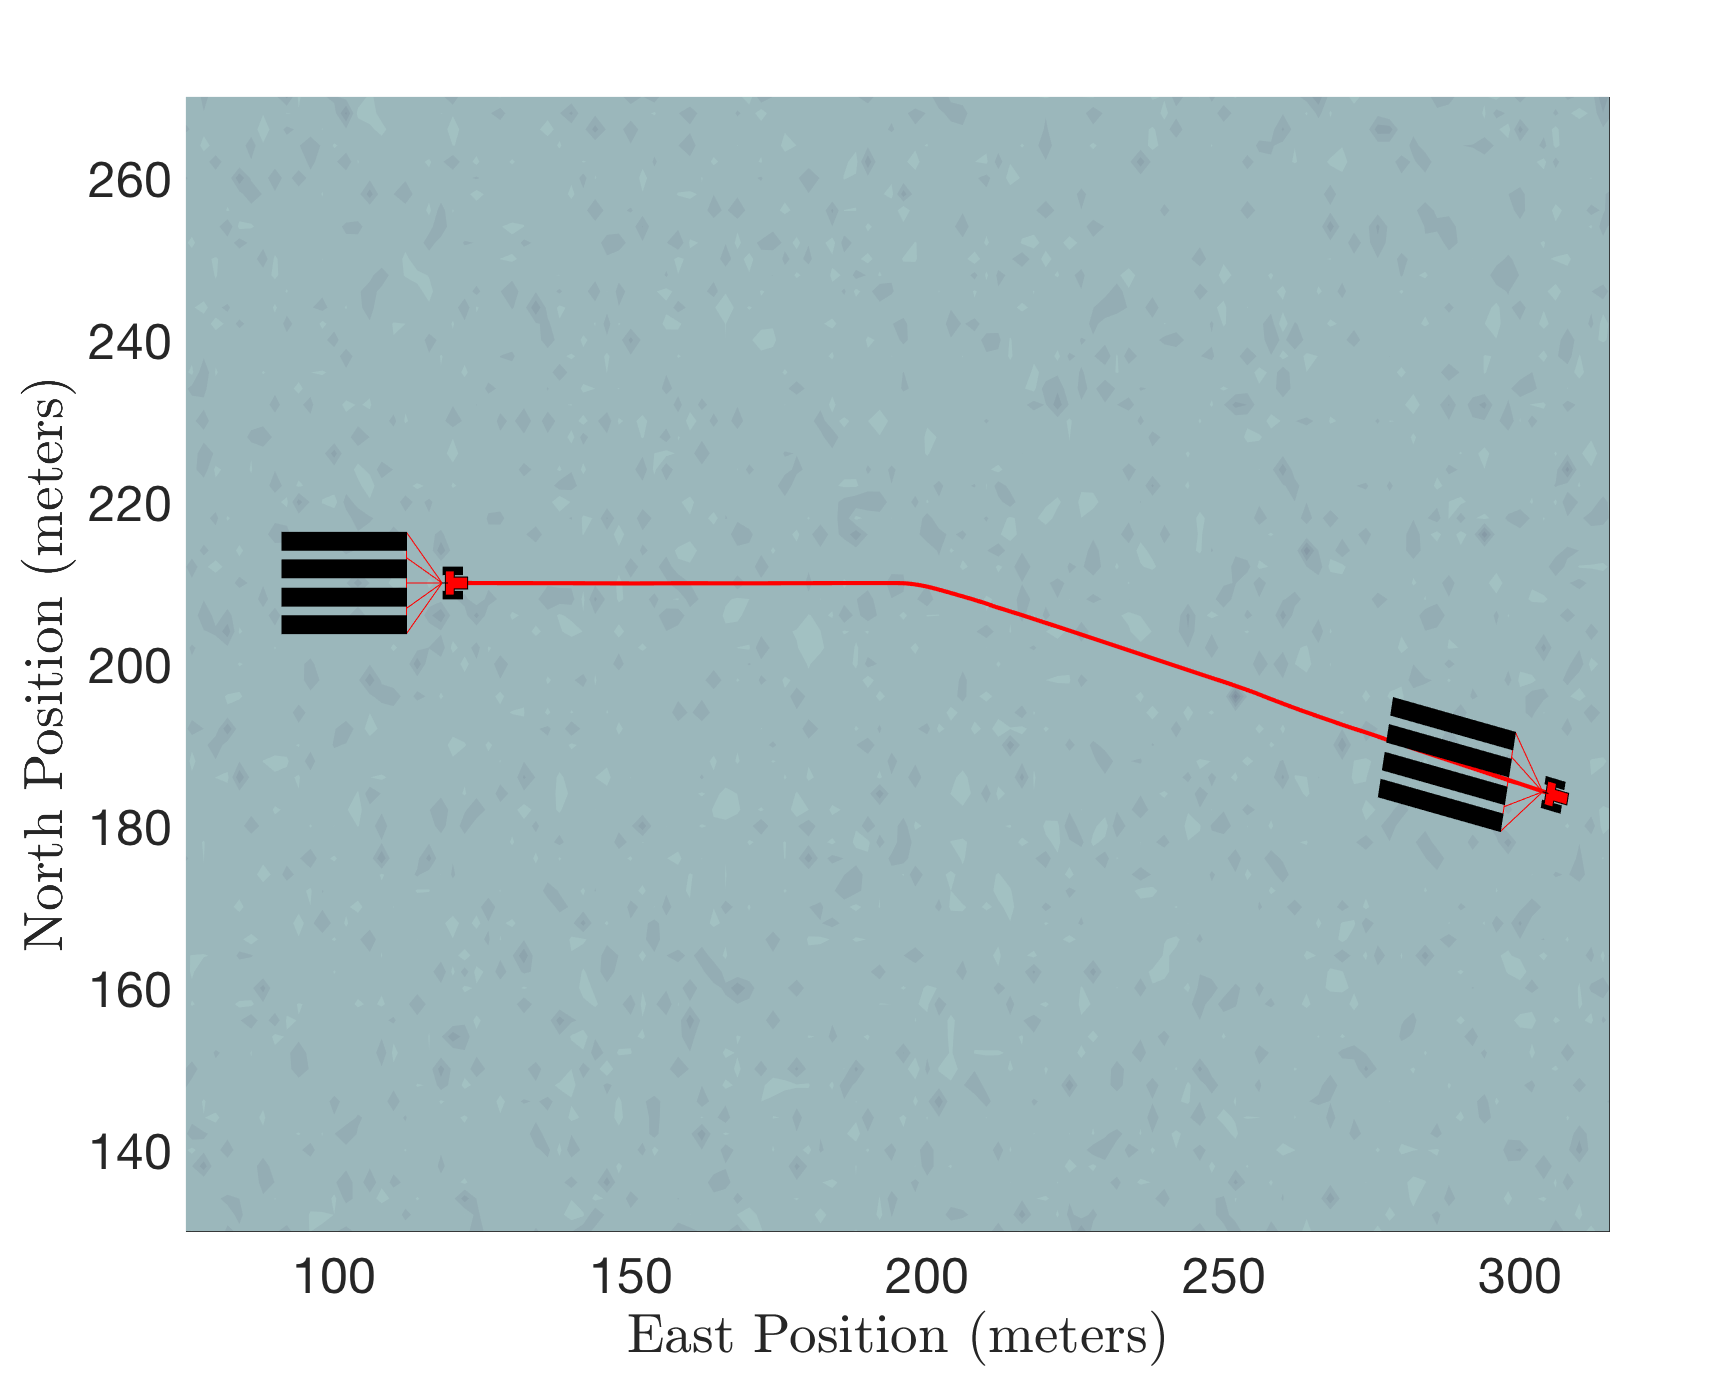
\includegraphics[width=4in]{RMBD_1Tractor_2DPlot}
    \caption{One tractor colored red and its 2D $[X, Y]$ location trajectory highlighted in red. The starting location is $[120, 210]$. A snapshot of the vehicle is taken at the starting and terminal locations of the simulation.}
    \label{fig:MB_Tractor_2D_Plot}
\end{figure}
\begin{figure}[htbp]
    \centering
    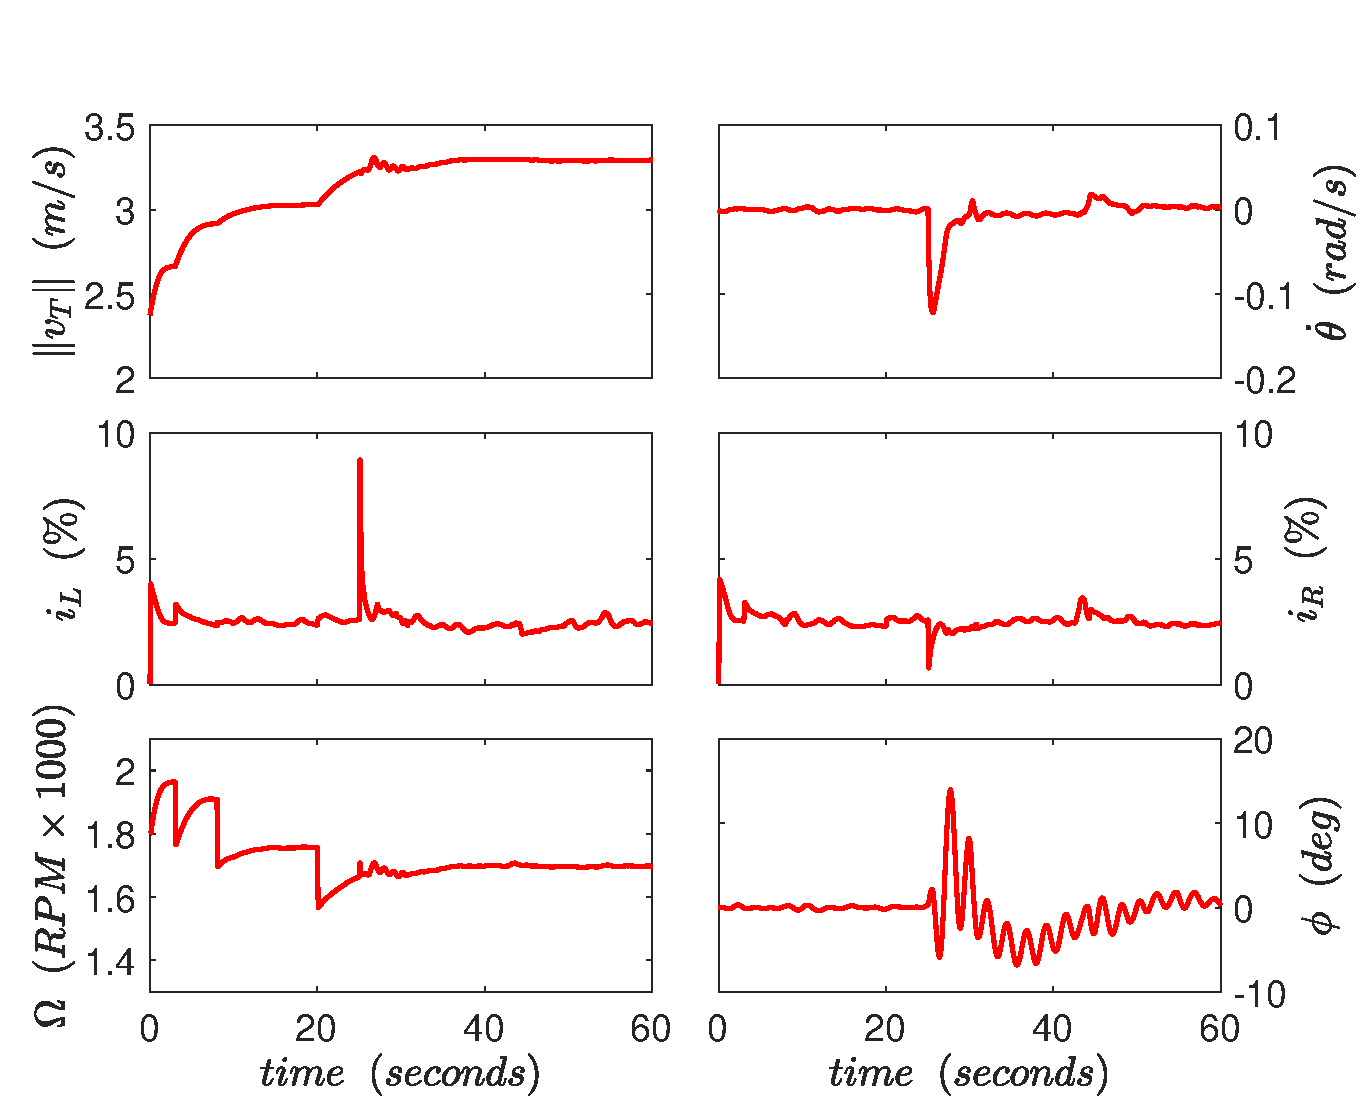
\includegraphics[width= 5.5in]{RMBD_1Tractor_Traj}
     \vspace{-5pt}
    \caption{Plots of vehicle speed $||v_T||$, yaw rate $\dot\theta$, left and right slip ratios $i_L$ and $i_R$, engine speed $\Omega$ and drawbar arm angle $\phi$ for the red tractor.}
     \vspace{-5pt}
    \label{fig:MB_Tractor_traj}
\end{figure} 
Closed-loop commands for heading are regulated using a PI contorller and generated using a sequence of two way points with $[X_{WP},Y_{WP}] = [210,1000]$ for $ t \in [0,20)$ seconds and $[X_{WP},Y_{WP}] = [20,1000]$ for $ t \in [20,60]$ where $X_{WP}$ and $Y_{WP}$ are the X and Y coordinates the tractor drives towards. Controller gains for tractor heading correction are $K_{p,\theta} = 2\frac{deg}{deg}$ and $K_{i,\theta} = 0.05\frac{deg}{deg}$. Initially the tractor drives straight but the second way point in the sequence forces it to take an abrupt right turn. This abrupt heading change excites the drawbar arm and elicits payload stability issues. These simulation results highlight the additional fidelity of the mulit-body model which will be valuable in developing controllers for the leader-follower control mode.
